%==============================================================
%  Which Data Fits Which Classifier?
%  An Object-Oriented Testbed for Model- and Domain-Specific
%  Data Suitability on Korean NLI
%
%  Compile: pdfLaTeX  (Overleaf recommended)
%    pdflatex main_en  ->  bibtex main_en  ->  pdflatex x2
%==============================================================
\documentclass[conference]{IEEEtran}

\usepackage[T1]{fontenc}
\usepackage{lmodern}
\usepackage[utf8]{inputenc}
\usepackage{amsmath,amssymb}
\usepackage{booktabs}
\usepackage{array}
\usepackage{graphicx}
\usepackage{tikz}
\usetikzlibrary{shapes.multipart, positioning, arrows.meta, calc}
\usepackage{listings}
\usepackage{xcolor}
\usepackage{url}
\usepackage{hyperref}

% ---- listing style for the OOP code excerpts ----
\lstset{
  basicstyle=\ttfamily\footnotesize,
  keywordstyle=\color{blue!70!black}\bfseries,
  commentstyle=\color{green!40!black}\itshape,
  stringstyle=\color{red!60!black},
  numbers=none,
  breaklines=true,
  breakatwhitespace=true,
  showstringspaces=false,
  language=Python,
  frame=single,
  framesep=4pt,
  xleftmargin=5pt,
  xrightmargin=3pt,
  aboveskip=12pt,
  belowskip=14pt,
  abovecaptionskip=2pt,
  belowcaptionskip=4pt,
}
% 캡션-프레임 및 프레임-본문 간격 (전역 기본값)
\setlength{\abovecaptionskip}{3pt}
\setlength{\belowcaptionskip}{6pt}
% 부동(float)이 아닌 lstlisting이 단/페이지 끝에서 잘리지 않도록 여유 확보
\setlength{\floatsep}{8pt plus 2pt minus 2pt}
\setlength{\textfloatsep}{10pt plus 2pt minus 2pt}

\begin{document}

\title{Which Data Fits Which Classifier? An Object-Oriented
Testbed for Model- and Domain-Specific Data Suitability on Korean NLI}

\author{
\IEEEauthorblockN{Dawon Lee}
\IEEEauthorblockA{Department of Computer Science and Engineering\\
Konkuk University, Seoul, Korea\\
rudaa1018@gmail.com}
}

\maketitle

%--------------------------------------------------------------
\begin{abstract}
A recurring intuition in machine learning practice is that different
classifiers, and different data domains, call for different training
data. We turn this intuition into a controlled, object-oriented
experiment on Korean Natural Language Inference (NLI). Three classifiers
---$k$-nearest neighbors (KNN), a neural network implemented from scratch
in NumPy, and a fine-tuned BERT---are built behind a single
\texttt{Classifier} abstraction so that they are mutually substitutable,
and a companion \texttt{Domain}/\texttt{TrainingStrategy} pair turns the
KLUE-NLI dataset into a target domain crossed with a training strategy,
under controlled low-data budgets. BERT dominates the
embedding-based classifiers. The central question---to perform well on a
target domain, should one train \emph{only} on that domain (targeted) or
on the whole pool (broad)?---is answered by evaluating each strategy on
augmenting a small in-domain baseline with either in-domain (targeted)
or whole-pool (broad) data: for a well-represented target the choice is
irrelevant, but for an under-represented one, in-domain augmentation is
more data-efficient per example but capped by the scarce pool; what
happens past that cap scales with model capacity---past the ceiling, broad
(off-domain) augmentation gains BERT $+0.037$ macro-F1 but KNN and NN only
$\approx +0.004$. Throughout, the accuracy--macro-F1 gap
exposes behavior that accuracy alone hides---the NumPy network inflates
accuracy by collapsing onto the easiest class. All findings are reported
as specific to this dataset; we make no claim of general superiority.
\end{abstract}

\begin{IEEEkeywords}
object-oriented design, natural language inference, Korean NLP,
$k$-nearest neighbors, neural networks, BERT, data suitability
\end{IEEEkeywords}

%--------------------------------------------------------------
\section{Introduction}
\label{sec:intro}

Practitioners routinely assume that the ``right'' training data depends
on \emph{what} is being trained: a nearest-neighbor model, a small
neural network, and a large pre-trained transformer are believed to
benefit from different data, and a model is believed to behave
differently across data domains. These assumptions are usually stated
informally. This paper makes them the subject of a controlled
experiment, and uses object-oriented (OO) design to keep that comparison
fair. The topic is chosen to align with the
author's intended direction in data-centric Korean NLP, where deciding
\emph{which data suits a given model} is a recurring and practical
question; building the comparison as a clean OO system is both the
course exercise and a small step toward that research interest.

This question also isolates one stage of a larger loop in generative
multi-agent systems. When such a system answers incorrectly, one would
first localize the fault to a particular agent (credit assignment) and
only then decide what data to feed \emph{that} agent. We take that
localization as given and probe the stage that follows it: once a single
agent has been singled out, should it be augmented only with data from
its own domain (\emph{targeted}) or from the shared pool (\emph{broad})?
The three classifiers stand in, by analogy, for such a single localized
agent under a fixed low-data budget. This paper is therefore a
deliberately small, controlled probe of that one decision with simplified
proxy models---not of the full multi-agent system, and not of the credit
assignment that precedes the decision.

We study Korean NLI---given a premise and a hypothesis, decide whether
the hypothesis is an \emph{entailment}, is \emph{neutral}, or is a
\emph{contradiction} of the premise. NLI is a useful probe because its
three-way label structure is shared by many downstream judgments, and
because the public KLUE-NLI benchmark \cite{park2021klue} annotates each
example with a \emph{source}, letting us carve out data domains in a
principled way.

Our contributions are two.
\begin{itemize}
  \item \textbf{(G1) A substitutable classifier hierarchy.}
        KNN, a from-scratch NumPy network, and a fine-tuned BERT are
        implemented behind one abstract \texttt{Classifier} interface.
        They satisfy the same contract (the Liskov Substitution
        Principle), and new classifiers are added as subclasses without
        touching the experiment loop (the Open--Closed Principle).
  \item \textbf{(G2) A target\,$\times$\,strategy design, evaluated per
        target.} Using \texttt{Domain} and \texttt{TrainingStrategy}
        abstractions, we ask whether training only on a target domain
        (\emph{targeted}) or on the whole pool (\emph{broad}) is better
        \emph{for that domain}, evaluating each on the target's own test
        slice at matched data volume. This avoids the
        test-composition artifact that a whole-set evaluation introduces.
\end{itemize}
Alongside these we report macro-F1 rather than accuracy throughout, which
exposes a model-specific behavior that accuracy alone hides (the NumPy
network's class-collapse); we treat this as a methodological choice
supporting the two contributions above, not as a separate contribution of
its own (Section~\ref{sec:pertarget}).

\paragraph*{Scope and stance}
We deliberately limit our claims. All quantitative results hold
\emph{for this dataset and this budget}; we do not assert that any model
is generally better. The three classifiers also serve, by
\emph{analogy}, as a proxy for a \emph{single} agent already singled out
by credit assignment---not for the routing or fault attribution that
precedes that point, and not claimed to be identical to any real
component. The single genuine technical bridge we draw (Section
\ref{sec:conclusion}) is that BERT-family sentence embeddings underlie
both our KNN/NN feature space and modern semantic-matching pipelines.

%--------------------------------------------------------------
\section{Related Work}
\label{sec:related}

\paragraph*{Object-oriented design}
Our class structure follows the classic strategy-pattern formulation of
the Gang of Four \cite{gamma1994design} and, concretely, the
nearest-neighbor case study of Lott and Phillips
\cite{lott2021python}, whose \texttt{Sample}/\texttt{TrainingData}
/\texttt{Hyperparameter} decomposition we adapt to sentence pairs and
generalize from a single distance rule to an abstract
\texttt{Classifier} family.

\paragraph*{Classifiers}
The three models are deliberately drawn from different eras and
inductive biases: instance-based nearest-neighbor classification
\cite{cover1967nearest}; the error back-propagation network
\cite{rumelhart1986learning}, which we re-implement in NumPy to expose
its forward and backward passes; and BERT \cite{devlin2019bert}, a
pre-trained bidirectional transformer fine-tuned end-to-end. For the
embedding-based models we encode sentences with Sentence-BERT
\cite{reimers2019sentence}, the siamese-network approach to producing
fixed-length sentence vectors. Standard evaluation conventions follow
common practice in the scikit-learn ecosystem \cite{pedregosa2011scikit},
although our metrics and neural network are implemented directly rather
than imported, since the OO design and the network internals are the
object of study.

\paragraph*{Korean NLI}
We use KLUE-NLI \cite{park2021klue}, part of the Korean Language
Understanding Evaluation benchmark, whose per-example source annotations
make a controlled domain split possible.

%--------------------------------------------------------------
\section{Proposed Object-Oriented System}
\label{sec:system}

\subsection{Two Axes: Model and Data}
The experiment has a \emph{model} axis (KNN, NN, BERT) and a \emph{data}
axis (which data a model is trained on). We treat the data axis with the
\texttt{Domain}/\texttt{TrainingStrategy} abstractions
(Section~\ref{sec:domains}) and evaluate every model \emph{per target
domain}---on the target's own test slice
(Section~\ref{sec:pertarget})---rather than on the whole validation set,
because a mixed test set would conflate the target with the test
composition. The model axis is then read directly off those same
per-target curves, where all three classifiers appear as rows
(Figure~\ref{fig:aug}). Throughout, two invariants keep comparisons
interpretable: training pools are label-balanced (so data \emph{kind}, not
class skew, varies), and the validation set is fixed (sliced by target for
the per-target view).

\subsection{Class Architecture}
Figure~\ref{fig:uml} sketches the class hierarchy. Data is modeled by an
encapsulated \texttt{NLISample} (two sentences) and its labeled subclass
\texttt{KnownNLI}, both built through a \texttt{from\_dict} factory that
raises a custom \texttt{InvalidSampleError} (a \texttt{ValueError}
subclass, chained with \texttt{raise\ldots from}) on malformed input.
The factory follows an EAFP style---it attempts the conversion and
catches the resulting \texttt{ValueError} rather than pre-checking every
field---and a \texttt{\_\_repr\_\_} gives samples a readable form for
debugging.
Representation is captured by an abstract \texttt{Embedder}; semantics
is captured by an abstract \texttt{Classifier}. Each concrete model is a
subclass, so adding a model or an embedding strategy means writing a new
subclass, not editing existing code.

\begin{figure*}[t]
\centering
\begin{tikzpicture}[
  umlclass/.style={
    draw, rectangle split, rectangle split parts=2,
    fill=blue!4, text width=2.5cm, align=left,
    font=\ttfamily\scriptsize, inner sep=3pt},
  abstractclass/.style={umlclass, fill=orange!10},
  inh/.style={-{Triangle[open, length=3mm, width=3mm]}, thick},
  use/.style={-{Stealth[length=2mm]}, dashed, gray!70!black},
  note/.style={font=\itshape\scriptsize, text width=3cm, align=center}]

% --- top row: data model + two abstractions ---
\node[umlclass] (sample) at (0,0)
  {\textbf{NLISample}\nodepart{second}+premise\\+hypothesis\\+from\_dict()\\+\_\_repr\_\_()};
\node[abstractclass] (emb) at (4.7,0)
  {\textbf{\guillemotleft abstract\guillemotright}\\\textbf{Embedder}\nodepart{second}+fit()*\\+embed()*\\+embed\_pair()*\\+dim*\\+embed\_many()$^\dagger$};
\node[abstractclass] (clf) at (11.6,0)
  {\textbf{\guillemotleft abstract\guillemotright}\\\textbf{Classifier}\nodepart{second}+fit()*\\+predict\_many()*\\+predict()$^\dagger$};

% --- second row: concrete subclasses ---
\node[umlclass] (known) at (0,-3.1)
  {\textbf{KnownNLI}\nodepart{second}+label\\+from\_dict()};
\node[umlclass] (sbert) at (4.7,-3.1)
  {\textbf{SBERTEmbedder}\nodepart{second}+embed\_many()\\$\phi=[u;v;$\\$\;|u\!-\!v|;u\!\odot\! v]$};
\node[umlclass] (knn) at (8.8,-3.3)
  {\textbf{KNNClassifier}\nodepart{second}-k : @property\\+predict\_many()};
\node[umlclass] (nn) at (11.6,-3.3)
  {\textbf{NNClassifier}\nodepart{second}-W1,-W2\\+fit() (NumPy)\\+predict\_many()};
\node[umlclass] (bert) at (14.4,-3.3)
  {\textbf{BertClassifier}\nodepart{second}-model\\+predict\_many()};
\node[umlclass] (err) at (0,-5.2)
  {\textbf{InvalidSampleError}\nodepart{second}(extends ValueError)};

% --- inheritance (hollow triangle) ---
\draw[inh] (known.north) -- (sample.south);
\draw[inh] (sbert.north) -- (emb.south);
\draw[inh] (knn.north) -- (clf.south);
\draw[inh] (nn.north) -- (clf.south);
\draw[inh] (bert.north) -- (clf.south);

% --- dependencies (dashed) ---
\draw[use] (sbert.west) -- node[above, font=\scriptsize]{encodes} (known.east);
\draw[use] (knn.west) -- node[above, font=\scriptsize]{uses $\phi$} (sbert.east);
\draw[use] (sample.west) -- ++(-0.45,0) |- node[pos=0.25, left, font=\scriptsize]{raises} (err.west);

\node[note] at (14.4,-5.4) {BertClassifier consumes raw text directly (self-attention), \emph{not} $\phi$};
\end{tikzpicture}
\caption{UML class diagram of the system. Hollow triangles denote
inheritance, dashed arrows denote dependency. In the two abstract
classes, $*$ marks abstract methods (which every subclass must
implement) and $\dagger$ marks a concrete default method provided by the
abstract class itself: \texttt{Embedder.embed\_many} stacks
\texttt{embed\_pair} one sample at a time and is overridden by
\texttt{SBERTEmbedder} for batch encoding, while
\texttt{Classifier.predict} wraps \texttt{predict\_many} for the
single-sample case. \texttt{KnownNLI} overrides \texttt{from\_dict} to
additionally parse its label. Two abstractions
(\texttt{Embedder}, \texttt{Classifier}) anchor the design: KNN, NN, and
BERT are interchangeable behind \texttt{Classifier} (Liskov
Substitution), and a new model or embedding is added purely as a new
subclass (Open--Closed). Note the asymmetry in data flow: KNN and NN
consume the SBERT relation vector $\phi(u,v)$, whereas BERT consumes the
raw \texttt{NLISample} text.}
\label{fig:uml}
\end{figure*}

Two design decisions make the diagram more than a drawing. First, the
\emph{experiment driver is model-agnostic}: it holds a list of
\texttt{Classifier} objects and calls \texttt{fit} and
\texttt{predict\_many} on each, never naming a concrete class. Because
every classifier honors the same contract, each cell of the grid is run
through the same two calls---\texttt{fit} then \texttt{predict\_many}---so
the harness treats all three models uniformly; the only difference is the
representation each consumes (embeddings for KNN/NN, raw text for BERT).
This uniform call site is the Liskov Substitution Principle in action.
Second, the two abstractions
\texttt{Embedder} and \texttt{Classifier} are deliberately
\emph{separate}: representation (how a sentence pair becomes numbers) is
decoupled from decision (how numbers become a label). A new embedding
strategy is a new \texttt{Embedder} subclass; a new model is a new
\texttt{Classifier} subclass; neither forces edits to the other or to
the driver, which is the Open--Closed Principle.

The diagram also makes the data flow explicit, and the asymmetry is
intentional. For KNN and NN the path is
\texttt{NLISample} $\rightarrow$ \texttt{Embedder} $\rightarrow$
\texttt{Classifier}: the sample is first turned into the relation vector
$\phi(u,v)$ and only then classified. For BERT the path is
\texttt{NLISample} $\rightarrow$ \texttt{Classifier} directly: there is
no \texttt{Embedder}, because the model learns its own representation.
The shared abstraction thus accommodates two genuinely different
pipelines without special-casing either. Table~\ref{tab:oop} summarizes
where each object-oriented mechanism is realized.

\begin{table}[t]
\centering
\footnotesize
\caption{Object-oriented mechanisms and where each is realized.}
\label{tab:oop}
% \arr: 줄바꿈이 허용되는 화살표 (긴 상속 체인이 칼럼 밖으로 넘치지 않도록)
\newcommand{\arr}{\,\allowbreak$\rightarrow$\,\allowbreak}
\begin{tabular}{@{}>{\raggedright\arraybackslash}p{1.95cm}>{\raggedright\arraybackslash}p{5.75cm}@{}}
\toprule
Mechanism & Realization in the system \\
\midrule
Encapsulation & \texttt{NLISample} stores and validates its two sentences; bad input never enters the pipeline. \\
Inheritance & \texttt{KnownNLI}\arr\texttt{NLISample}; the three classifiers\arr\texttt{Classifier}; \texttt{SBERTEmbedder}\arr\texttt{Embedder}; \texttt{SourceSetDomain}/ \texttt{UniverseDomain}\arr\texttt{Domain}; the two strategies\arr\texttt{TrainingStrategy}. \\
Abstraction & \texttt{Embedder} and \texttt{Classifier} are ABCs that fix a contract without an implementation. \\
Polymorphism (Strategy) & the driver calls \texttt{predict\_many} on any \texttt{Classifier}; dispatch picks the right body. \\
Factory method & \texttt{from\_dict} constructs samples from raw rows. \\
Custom exception & \texttt{InvalidSampleError(ValueError)}, chained with \texttt{raise\,\ldots\,from}. \\
EAFP & \texttt{from\_dict} attempts the conversion and catches \texttt{ValueError}, rather than pre-checking every field. \\
Magic methods & \texttt{\_\_repr\_\_} gives samples a debuggable string form. \\
Property & \texttt{@property k} with a validating setter on \texttt{KNNClassifier}. \\
Parameterization & formal/colloquial are \emph{instances} of one \texttt{SourceSetDomain}, not per-domain subclasses. \\
LSP & all three classifiers are interchangeable behind \texttt{Classifier}. \\
OCP & a new model or embedding is a new subclass; the driver is untouched. \\
\bottomrule
\end{tabular}
\end{table}

\subsection{Embedding Layer (KNN/NN)}
The instance-based and shallow-neural models cannot ingest raw text, so
an \texttt{SBERTEmbedder} encodes the premise $u$ and hypothesis $v$
separately with a Korean Sentence-BERT model and combines them into a
single relation vector
\begin{equation}
\phi(u,v) = [\,u\ ;\ v\ ;\ |u-v|\ ;\ u\odot v\,],
\end{equation}
where $|u-v|$ and $u\odot v$ are the standard difference and
element-wise product features that make the pair's \emph{relation}
explicit. With a 768-dimensional base encoder this yields a
3072-dimensional input. \texttt{KNNClassifier} consumes $\phi$ directly:
it $L_2$-normalizes the relation vectors and classifies a query by
majority vote over its $k$ nearest neighbors under \emph{cosine
similarity}, computed directly rather than through a library distance
routine, with $k$ selected on the development split.

\subsection{NumPy Neural Network}
\texttt{NNClassifier} is a one-hidden-layer network whose forward and
backward passes are written by hand, with no autograd. Inputs are
standardized; weights use He initialization; the hidden activation is
ReLU and the output is a softmax trained with cross-entropy. With
one-hot targets $Y$ and predicted probabilities $P$, the gradients are
\begin{align}
\delta_2 &= (P-Y)/m, &
\nabla_{W_2} &= a_1^{\top}\delta_2 + \lambda W_2, \\
\delta_1 &= (\delta_2 W_2^{\top})\odot \mathbf{1}[z_1>0], &
\nabla_{W_1} &= X^{\top}\delta_1 + \lambda W_1,
\end{align}
optimized by momentum SGD with $L_2$ weight decay $\lambda$. Building
the network this way keeps the \emph{implementation} of learning---not
merely its use---inside the object-oriented design. Listing~\ref{lst:core}
shows the abstract contract together with the hand-written backward pass.

\begin{lstlisting}[caption={Core implementation: the abstract
\texttt{Classifier} contract and the from-scratch backward pass of
\texttt{NNClassifier}.}, label={lst:core}]
class Classifier(ABC):
    @abstractmethod
    def fit(self, X, y): ...
    @abstractmethod
    def predict_many(self, X): ...
    def predict(self, x):           # shared default
        return int(self.predict_many(x[None])[0])

class NNClassifier(Classifier):
    def _backward(self, xb, yb, z1, a1, p, m):
        dz2 = (p - yb) / m                       # softmax + CE
        dW2 = a1.T @ dz2 + self.l2 * self.W2
        dz1 = (dz2 @ self.W2.T) * (z1 > 0)       # ReLU grad
        dW1 = xb.T @ dz1 + self.l2 * self.W1
        return dW1, dW2                          # + biases
\end{lstlisting}

\subsection{BERT Classifier (Self-Representation)}
\texttt{BertClassifier} is the third \texttt{Classifier} subclass, but it
differs in kind: it does \emph{not} consume the SBERT embedding. It
tokenizes the raw premise--hypothesis pair and fine-tunes
\texttt{klue/bert-base} end-to-end, learning its own representation and
modeling token-level interaction between the two sentences through
self-attention. This contrast is itself part of the argument: under one
\texttt{Classifier} abstraction, KNN and NN depend on an external
sentence representation, whereas BERT learns one---so ``the data each
model sees'' is not the same kind of object across the hierarchy.

\subsection{Domain and Strategy Abstractions}
\label{sec:domains}
The experiment's \emph{data} axis is given the same object-oriented
treatment as its models. A \texttt{Domain} is a set of sources that plays
two roles at once: it selects a training pool and it defines a test slice
(\texttt{test\_mask}). Here a single concrete \texttt{SourceSetDomain}
holds its source set as data, so the formal and colloquial domains are
two \emph{instances} of that one class---\texttt{FORMAL\_DOMAIN} over
the written-register sources and \texttt{COLLOQUIAL\_DOMAIN} over the
spoken-register ones---rather than two separate subclasses; a
\texttt{UniverseDomain} that contains every source is the only other
concrete \texttt{Domain}. Parameterizing by a source set instead of
subclassing per domain is a deliberate choice: it keeps the hierarchy
flat and adds a new domain by constructing an object, not by writing a
class. On
top of this, a \texttt{TrainingStrategy} decides, given a target domain,
which pool to train on---a textbook Strategy pattern (Listing~\ref{lst:strategy}).
\texttt{TargetedStrategy} returns the target itself (train in-domain);
\texttt{BroadStrategy} returns the universe (train on everything). The
``target $\times$ strategy'' experiment of Section~\ref{sec:pertarget} is
then nothing but iterating two domains over two strategies, with the
correct test slice chosen automatically by the target domain. Adding a
third domain is a new \texttt{SourceSetDomain} \emph{instance}, and a
third strategy is a new \texttt{TrainingStrategy} subclass.

\begin{lstlisting}[caption={The data axis as objects: a \texttt{Domain}
is both a training pool and a test slice; the formal and colloquial
domains are two \emph{instances} of one parameterized
\texttt{SourceSetDomain}; a \texttt{TrainingStrategy} maps a target to a
training pool.}, label={lst:strategy}]
class Domain(ABC):
    @abstractmethod
    def contains(self, source): ...
    def test_mask(self, sources):     # eval slice
        return np.array([self.contains(s) for s in sources])

class SourceSetDomain(Domain):        # parameterized, not subclassed per domain
    def __init__(self, name, sources):
        self._name, self.sources = name, set(sources)
    def contains(self, source):
        return source in self.sources

FORMAL     = SourceSetDomain("formal", {"wikipedia", ...})
COLLOQUIAL = SourceSetDomain("colloquial", {"NSMC", "airbnb"})

class TrainingStrategy(ABC):
    @abstractmethod
    def pool(self, target): ...

class TargetedStrategy(TrainingStrategy):
    def pool(self, target): return target        # in-domain
class BroadStrategy(TrainingStrategy):
    def __init__(self, universe): self._u = universe
    def pool(self, target): return self._u       # everything
\end{lstlisting}

%--------------------------------------------------------------
\section{Experimental Setup}
\label{sec:setup}

\paragraph*{Dataset and domains}
KLUE-NLI \cite{park2021klue} provides 24{,}998 training and 3{,}000
validation premise--hypothesis pairs labeled entailment / neutral /
contradiction. Each training example carries a \emph{source}. We define a
\textbf{formal} domain from the written-register sources
(\texttt{wikipedia}, \texttt{wikinews}, \texttt{wikitree},
\texttt{policy}), a \textbf{colloquial} domain from the spoken-register
review sources (\texttt{NSMC}, movie reviews; \texttt{airbnb}, lodging
reviews), and treat their union as the \textbf{combined} (universe) pool.
The validation set carries sources too, so each domain also defines a
test slice: $1{,}800$ formal and $1{,}200$ colloquial of the $3{,}000$
validation examples.

\paragraph*{Targets and strategies}
Each target starts from a small $2{,}000$-example in-domain baseline and
is \emph{augmented}, adding either targeted (in-domain) or broad
(whole-pool) data at matched volume, evaluated on the target's own test
slice. Sweeping the augmented size from $2{,}000$ to $14{,}000$ traces a
data-efficiency curve; targeted augmentation is bounded by the target's
in-domain pool, so the colloquial targeted arm reaches its last feasible
checkpoint near $8{,}000$ as its $\approx 9{,}000$-example pool runs out,
whereas the formal target (pool $\approx 15{,}000$) and all broad arms
continue to $14{,}000$. All three models are
evaluated \emph{incrementally}: from the baseline, data is added in order
up to the pool limit and the validation metric is checkpointed at each
size, rather than retraining independently per size. Every curve is the
mean of $8$ seeds (BERT at considerable cost), and the figure shows
$\pm$one standard deviation as a band.

\paragraph*{Hyperparameters without test leakage}
Every model's key hyperparameters are selected on a $20\%$ development
split held out from the training set, never on the validation set: the
neighbor count $k$ for KNN, the learning rate (over
$\{0.003, 0.01, 0.03, 0.1\}$) and number of epochs for the NumPy network,
and the fine-tuning rate (over $\{2,3,5\}\times10^{-5}$) for BERT, which
dev selection set to $3\times10^{-5}$. Crucially, the dev-based search for
the network also rejects any learning rate that numerically diverges, so
it is \emph{tuned}, not crippled by a fixed rate. The validation set is
touched only for the final reported numbers.

\paragraph*{Implementation}
All experiments run on an Apple M3 (Metal Performance Shaders backend).
KNN and NN consume Korean Sentence-BERT embeddings
(\texttt{jhgan/ko-sroberta-multitask}); BERT fine-tunes
\texttt{klue/bert-base}. The Sentence-BERT model is intentionally
general-purpose rather than KLUE-NLI-tuned, so as not to inflate the
embedding-based classifiers. Distances, the neural network, and all
metrics (accuracy, per-class precision/recall/F1, macro-F1, confusion
matrices) are implemented directly.

%--------------------------------------------------------------
\section{Implementation and Results}
\label{sec:results}

\subsection{Usage}
The whole hierarchy is exercised through the same two methods on every
model; only the representation differs. Listing~\ref{lst:usage} shows the
driver, and Listing~\ref{lst:console} the resulting console output of one
full run.\footnote{Source code and the executable notebook are available
at: \url{https://github.com/your-id/oop-nli} (replace with your repository, optional).}

\begin{lstlisting}[caption={Driving the three classifiers through one
uniform interface (\texttt{fit}/\texttt{predict\_many}).}, label={lst:usage}]
knn  = KNNClassifier(k).fit(X_tr, y_tr)      # embeddings
nn   = NNClassifier(ep).fit(X_tr, y_tr)      # embeddings
bert = BertClassifier().fit(samples, y_tr)   # raw text

for clf, X in [(knn, X_val), (nn, X_val),
               (bert, val_samples)]:
    acc, f1 = evaluate(y_val, clf.predict_many(X))
\end{lstlisting}

\begin{lstlisting}[language=, basicstyle=\ttfamily\scriptsize,
caption={Abridged console output: augmentation-curve checkpoints on the
colloquial target, macro-F1 (targeted / broad, mean of 8 seeds).},
label={lst:console}]
=== colloquial target, macro-F1 (targeted / broad) ===
  total= 6000   KNN .562/.551   NN .604/.585   BERT .722/.715
  total= 8000   KNN .564/.560   NN .618/.601   BERT .733/.719
  total=14000   KNN  -- /.568   NN  -- /.622   BERT  -- /.770
                (targeted pool exhausted ~9000; broad continues)
\end{lstlisting}

\subsection{Results: Augmenting a Low-Data Baseline}
\label{sec:pertarget}
We start each target from a deliberately small baseline of $2{,}000$
in-domain examples---a regime far from saturation, where data choices can
matter---and \emph{augment} it toward larger sizes. At each size the added
examples are drawn either from the target pool (\textbf{targeted},
in-domain augmentation) or from the whole pool (\textbf{broad}); both arms
share the same baseline and add the same number of examples, so only the
\emph{composition} of the augmentation differs. Each arm is evaluated on
the target's own test slice over $8$ seeds. Figure~\ref{fig:aug} shows the
curves for all three models.

\begin{figure}[t]
\centering
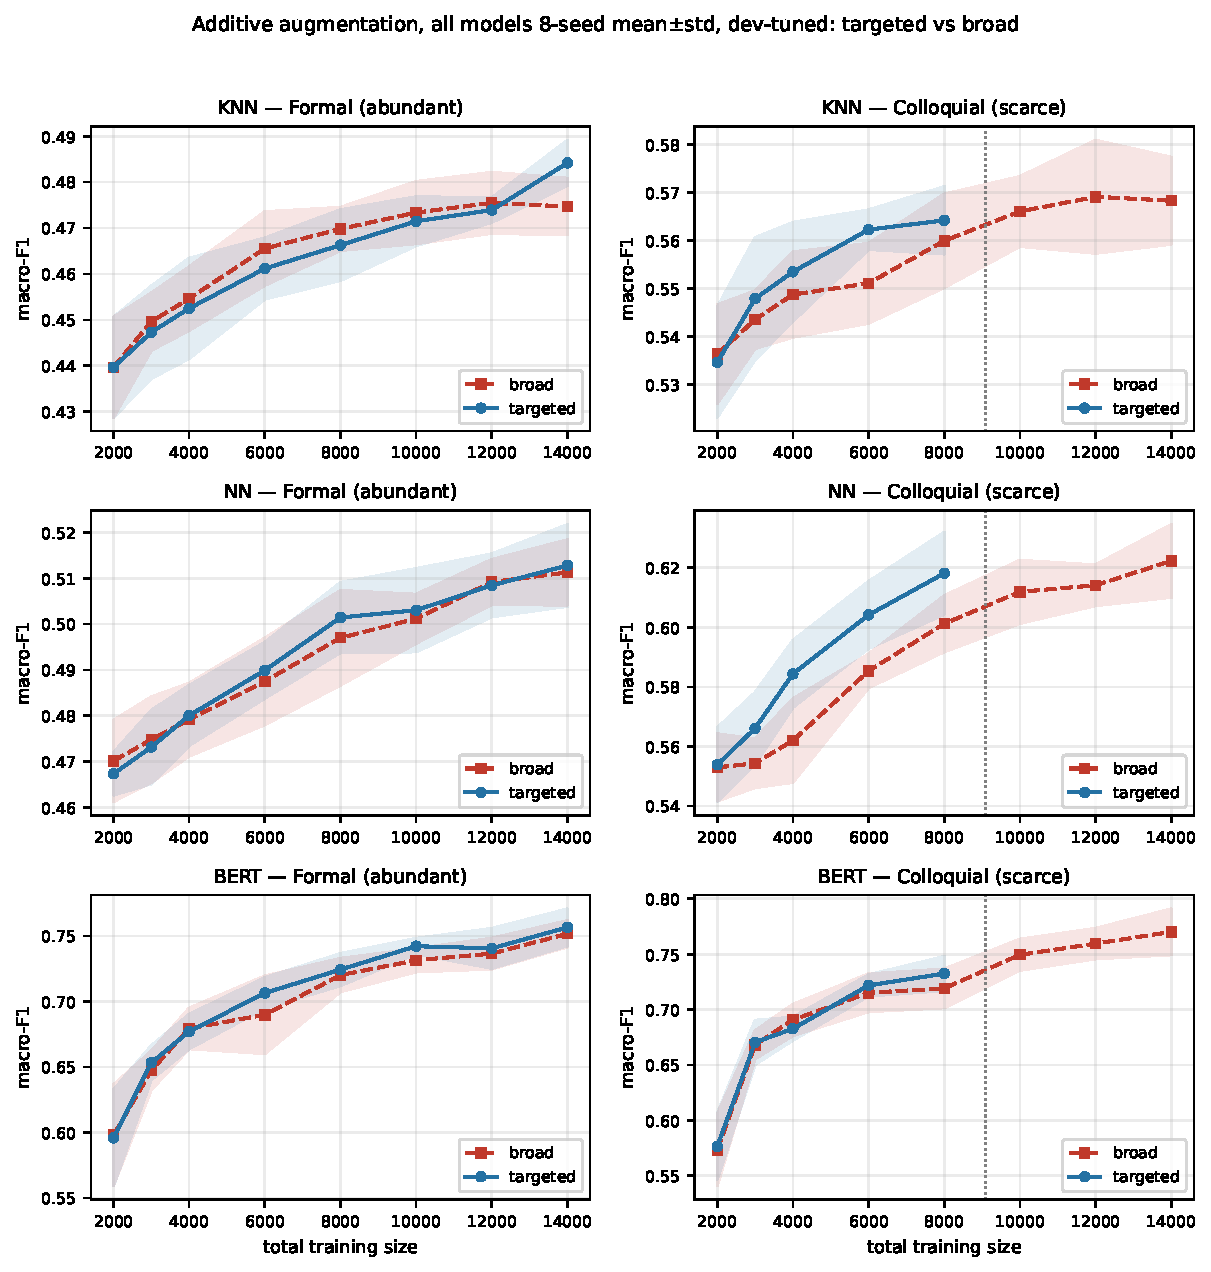
\includegraphics[width=\linewidth]{fig_augmentation.pdf}
\caption{Additive augmentation from a $2{,}000$-example baseline: targeted
(in-domain) vs.\ broad (whole-pool), for KNN, NN, BERT (rows). Each curve
is the mean$\pm$std of $8$ seeds with all hyperparameters dev-selected,
read by incremental checkpoints. At a matched size targeted is at least as
efficient; the targeted pool runs out near $9{,}000$, and past that broad
helps \emph{in proportion to capacity}---BERT gains $+0.037$ macro-F1 from
$8$k to $14$k while KNN and NN gain only $\approx +0.004$.}
\label{fig:aug}
\end{figure}

Three findings stand out; we read them through two-sample (Welch)
$t$-tests across the $8$ seeds per arm, computed from the per-size
mean and standard deviation (significance at $|t|>2.1$, $\alpha\approx.05$). \textbf{(i) For
the abundant domain, augmentation composition is irrelevant.} On the
formal target all three models reach essentially the same level whether
augmented in-domain or broadly: $22$ of the $24$ size$\times$model
comparisons are non-significant, and the two that reach nominal
significance (KNN at $14{,}000$, $|t|=3.4$; BERT at $10{,}000$, $|t|=2.8$)
involve effects of only ${\le}0.011$ macro-F1, fail Bonferroni correction,
and follow no consistent direction---the KNN point even has the opposite
sign to that model's other seven sizes. Since $\alpha=.05$ over $24$ tests
already expects ${\approx}1.2$ false positives, the formal result is
indistinguishable from no effect, and we read the composition difference
there as practically negligible rather than strictly null. \textbf{(ii) For the scarce
domain, in-domain data is more efficient at a matched size, but only for
the embedding-based models.} On the colloquial target at $6{,}000$,
targeted beats broad significantly for NN ($+0.019$, $t=4.2$) and KNN
($+0.011$, $t=3.4$); for BERT the gap is positive but within seed noise
($+0.007$, $t=1.0$, not significant). Targeted then runs out at the
in-domain pool's ceiling ($\approx 9{,}000$). \textbf{(iii) Past that
ceiling, the value of further (broad) augmentation scales with model
capacity.} Extending from targeted's last feasible size ($8{,}000$) to
broad at $14{,}000$ adds $6{,}000$ examples; that \emph{same} increment
raises BERT by $+0.037$ macro-F1 ($0.733\to0.770$, $t=4.1$) but KNN and NN
by only $+0.004$ each ($|t|<1$). Normalized to each model's remaining
head-room toward a perfect score, the gap is starker still---BERT closes
about $14\%$ of that distance against ${\approx}1\%$ for KNN and NN---so the
raw difference, if anything, understates it. Because the increment is
identical across models, the contrast is not a data-volume effect: a model that learns its
own representation extracts real signal from extra off-domain data, while
one on a frozen embedding barely does. Under Bonferroni correction over the
full family (${\sim}40$ targeted-vs-broad tests, $\alpha\approx.0013$,
$|t|>4.0$), only the NN matched-size advantage ($t=4.2$) and the BERT
capacity gap ($t=4.1$) survive; KNN's matched-size edge ($t=3.4$) and the
two formal blips do not. The
significant effects are large in standardized terms (Cohen's
$d\approx1.4$--$2.1$) yet small in absolute terms ($1$--$2$ macro-F1
points), the seed variance being tiny. Every model is tuned and averaged
identically (hyperparameters dev-selected---KNN's $k$, NN's learning rate
over $\{0.003,\dots,0.1\}$ rejecting rates that diverge, and BERT's set to
$3\times10^{-5}$---each curve the mean of $8$ seeds), so the comparison is
fair. In one line: \emph{in-domain augmentation is the more efficient
choice per example for a low-capacity model, but only a high-capacity
model keeps benefiting once one must augment with off-domain data.}

\paragraph*{Reading behavior beyond accuracy}
We read every curve above on macro-F1 rather than accuracy because the two
diverge in a model-specific way. The NumPy network can lift its raw
accuracy by over-predicting the easiest class, a collapse that
macro-F1---weighting all three classes equally---penalizes but accuracy
masks; tracking per-class precision and recall alongside macro-F1 is what
makes the degeneracy visible. This is a reporting discipline, not a finding
in itself, but it is the reason none of the comparisons above are read on
accuracy.

%--------------------------------------------------------------
\section{Limitations}
\label{sec:limits}

Several limits bound our claims. First, every number is specific to
KLUE-NLI and to a frozen, general-purpose sentence embedding; we sweep
eight seeds and a wide range of augmentation sizes but not multiple
datasets or encoders, so the conditional finding---in-domain augmentation
helps the \emph{under-represented} target---still needs external
replication. The effect is also modest in absolute size ($1$--$2$ macro-F1
points), and clearest on the embedding-based models (KNN and NN), whose
hyperparameters are dev-selected so the curves reflect tuned, not
crippled, learners. Second, collapsing a premise and a
hypothesis into a single vector $\phi(u,v)$ discards part of the
token-level interaction that a joint-attention model such as BERT can
exploit; this is a structural disadvantage of the embedding-based
classifiers and one lens on the BERT--vs--embedding gap, not a flaw to
be tuned away. Third, our evidence for the Liskov Substitution and
Open--Closed principles is at the level of design---the same loop drives
all three classifiers, and each was added as a subclass---rather than a
quantitative maintainability measurement, which is outside our scope.

Each limitation suggests a concrete improvement. The single-vector
$\phi(u,v)$ could be replaced by a cross-encoder \texttt{Embedder}
subclass that attends over both sentences---an addition that the
Open--Closed design admits without touching the classifiers. The
data-bound results could be hardened by sweeping seeds and budgets, and
by adding more \texttt{Classifier} subclasses (e.g., logistic regression,
a deeper network). Finally, the maintainability claim could be made
quantitative by measuring the lines changed when adding a new model---a
direct test of the Open--Closed Principle.

%--------------------------------------------------------------
\section{Conclusion}
\label{sec:conclusion}

We built an object-oriented testbed in which three classifiers behind a
single \texttt{Classifier} abstraction, and two data strategies behind a
\texttt{Domain}/\texttt{TrainingStrategy} pair, are compared on Korean
NLI. Augmenting a small in-domain baseline and evaluating on each target's
own test slice, we found that for an abundant target the augmentation
composition makes no practical difference (the few nominally significant
points are noise-level and survive no correction), and for a scarce target
the matched-size in-domain advantage is small and confined to the
lower-capacity models (NN and KNN, not BERT) before the scarce pool caps
it. The clearest effect---and the only one to survive multiple-comparison
correction---appears past that cap: the marginal value of broad
(off-domain) augmentation scales with capacity, so the high-capacity BERT
gains $+0.037$ macro-F1 (about $14\%$ of its remaining head-room) while KNN
and NN gain only $\approx +0.004$. Reporting macro-F1, not accuracy alone,
was essential to see this.

The broader motivation is data \emph{suitability}: asking not which
model is best in the abstract, but which data fits which classifier
under fair control. This mirrors a question in generative multi-agent
systems---augment each heterogeneous agent with data targeted to
\emph{its} weaknesses, or augment a shared pool?---of which our
targeted-vs-broad comparison is a first, deliberately small, controlled
instance (the classifiers remaining proxies for such agents by analogy,
not identity). The one concrete technical link is that BERT-family
sentence embeddings, which power our KNN/NN feature space, are also the
backbone of modern semantic-matching components; extending this
controlled comparison---more seeds, real synthetic augmentation, and
genuinely agent-specific weaknesses---is left as future work.

\paragraph*{Lessons learned}
Building the project taught three concrete object-oriented lessons.
First, abstraction paid for itself: defining \texttt{Classifier} once let
three very different models---an instance-based learner, a hand-written
network, and a fine-tuned transformer---share the same evaluation code,
and the experiment grew by adding subclasses rather than rewriting the
driver. Second, the abstraction's \emph{boundary} was instructive: KNN
and NN consume an \texttt{Embedder} output while BERT consumes raw text,
which showed that a shared interface can unify the \emph{call site} even
when the underlying representation differs---and that forcing the two
into one identical signature would have been a worse design than honestly
letting each consume what it needs. Third, the small disciplines mattered
in practice: a \texttt{from\_dict} factory with a custom
\texttt{InvalidSampleError} caught malformed rows before they reached the
models, and implementing back-propagation by hand---rather than calling a
library---turned the network from a black box into something I could
reason about and debug.

%--------------------------------------------------------------
\bibliographystyle{IEEEtran}
\bibliography{refs}

\end{document}
